\documentclass[12pt]{beamer}

\usepackage{ifluatex}
\ifluatex
  \usepackage[utf8]{luainputenc}
\else
  \usepackage[utf8]{inputenc}
\fi
\usepackage[ngerman]{babel}
\usepackage{amsmath}
\usepackage{cite}
\usepackage{siunitx}
\usepackage[compatibility=false]{caption}
\usepackage{subcaption}
\usepackage{colortbl}
\usepackage{epstopdf}
\usepackage{listings}

% Configure listings
\lstset{
%  moredelim=[is][\underbar]{_}{_},
  keepspaces=true,
  escapechar=§,
  breaklines=true,
  basicstyle=\footnotesize,
  commentstyle=\color{mygreen},
  keywordstyle=\color{blue},
  stringstyle=\color{mymauve},
  tabsize=4
}

\newcommand{\captionsource}[1]{\center\scriptsize [#1]}

\title{Optimierung biologisch-realistischer Neuronenmodelle}
\subtitle{Bachelor Projekt 2014}
\author{L. Weckeck \and L. Schiffer \and M. Spolert \and N. Kohlmorgen \and K. Buss \and F. Esch}
\institute{
  Institut für Robotik und Kognitive Systeme\\
  Universität zu Lübeck
}
\date{Betreuer: Christoph Metzner}
\subject{Neuronensimulation}
\usetheme{Frankfurt}
\usecolortheme{seahorse}
\definecolor{light-gray}{gray}{0.7}

\begin{document}

\begin{frame}
  \titlepage
\end{frame}

\begin{frame}
  \frametitle{Inhalt}
  \tableofcontents
\end{frame}

\section{Einleitung}

\subsection{Übersicht}

\begin{frame}
  \frametitle{Übersicht}
  \begin{itemize}
  \item Ziel: Leitfähigkeiten der Ionenkanäle optimieren
  \item Basis: Bachelorarbeit von Anne Kloskowki
  \item Erreicht:
    \begin{itemize}
    \item alternative Algorithmen und Konfigurationen
    \item GUI
    \item schnellerer Code; Nebenläufigkeit von Konfigurationen
    \item persistente Ausgabe (Datei, Zeitstempel)
    \end{itemize}
  \end{itemize}
\end{frame}


\subsection{Neuronenmodelle}

\begin{frame}
  \frametitle{Die Neuronenklassen}
  \scriptsize
  \begin{figure}
    \begin{subfigure}{.5\textwidth}
      \centering
      \includegraphics*[width=0.7\linewidth]{genetic/nowak-rs.png}
      \caption*{Regulär feuernd (RS)}
    \end{subfigure}%
    \begin{subfigure}{.5\textwidth}
      \centering
      \includegraphics*[width=0.7\linewidth]{genetic/nowak-fs.png}
      \caption*{Schnell feuernd (FS)}
    \end{subfigure}
  \end{figure}

  \begin{figure}
    \begin{subfigure}{.5\textwidth}
      \centering
      \includegraphics*[width=0.7\linewidth]{genetic/nowak-ib.png}
      \caption*{Intrinsisch burstend (IB)}
    \end{subfigure}%
    \begin{subfigure}{.5\textwidth}
      \centering
      \includegraphics*[width=0.7\linewidth]{genetic/nowak-ch.png}
      \caption*{Schnell rhytmisch burstend (CH)}
    \end{subfigure}
  \end{figure}
  {\scriptsize [Nowak et al., 2003]}
\end{frame}


\section{Entwicklung}

\subsection{Organisation}

\begin{frame}
  \frametitle{Organisation}
  \begin{itemize}
  \item Projektplan \\
    \begin{tabular}[H]{rl}
      Dauer & Phase \\ \hline
      2W & Einarbeitung \\
      3W & Implementierung \\
      1W & GUI \\
      3W & Evaluation \\
      1W & Vorbereitung: Präsentation
    \end{tabular}
  \item Versionsverwaltung: Git (Github)
  \item Arbeitszuteilung via Ticketsystem
  \item Styleguide: PEP 8
  \end{itemize}
\end{frame}

\subsection{Features}

\begin{frame}
  \frametitle{Konfigurationen}
  \begin{itemize}
  \item Problem: Einstellungen aufwändig/fehleranfällig
  \item<2-> Lösung: Konfig-Dateien
    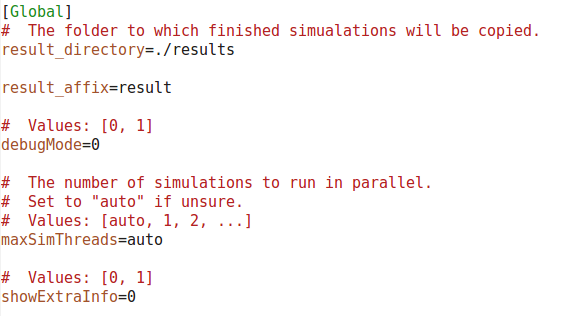
\includegraphics[width=0.6\textwidth]{config-example.png}
  \end{itemize}
\end{frame}

\begin{frame}
  \frametitle{Nebenläufigkeit}

  \begin{itemize}
  \item Probleme
    \begin{itemize}
    \item gemeinsame Dateien $\rightarrow$ ein Lauf pro Installation
    \item keine persistente Ausgabe
    \end{itemize}
  \item<2-> Lösung
    \begin{itemize}
    \item ``out of source'' Simulation (Pfad: results/)
    \item Logging dateien mit Zeitstempel.
    \end{itemize}

  \end{itemize}
\end{frame}

\section{Genetischer Algorithmus}

\subsection{Einleitung}

\begin{frame}
  \frametitle{Genetischer Algorithmus}
  \begin{columns}[T]
    \begin{column}{0.35\textwidth}
      \begin{itemize}
      \item Idee: biologische Evolution
      \item effizient bei komplexen Fitness Beziehungen
      \item Überwindung lokaler Maxima
      \end{itemize}
    \end{column}
    \begin{column}{0.65\textwidth}
        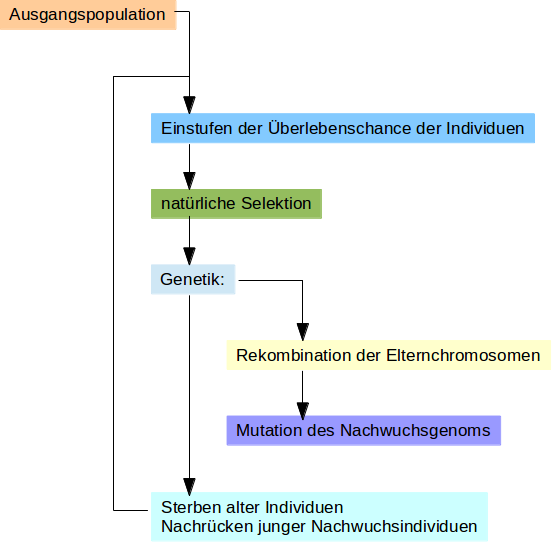
\includegraphics[width=\textwidth]{GenAlg-Diagramm.png}
        \captionsource{\tiny Evolutionäre Algorithmen zur Parametereinstellung
          in elektrophysiologischen Neuronenmodellen, Anne Kloskowski, 2013}
    \end{column}
  \end{columns}
\end{frame}


\subsection{GUI}

\begin{frame}
  \frametitle{GUI}
  \begin{block}{Features}
    \begin{itemize}
    \item Speichern/Laden von Konfigurationen
    \item Auswahl des Algorithmus'
    \item Einstellung der Parameter
    \end{itemize}
  \end{block}
  \only<2->{
    \center
    \LARGE
    Anwendungsbeispiel
  }
\end{frame}

\subsection{Ergebnisse}

\begin{frame}
  \frametitle{Durchführung}
  \begin{itemize}
  \item 44 Simulationen
  \item eine Baseline je Neuronklasse
    \scriptsize
    \begin{tabular}[H]{ll}
      Parameter & Werte \\\hline
      Populationsgröße & 50, 125, 200 \\ \arrayrulecolor{light-gray}\hline
      Tournament Selection, Tournamentgröße & 5, 15 \\
      Fitness Proportionate Selection & \\
      Truncation Selection  & \\ \hline
      Mutationsstärke & 0.08333, 0.15, 0.25 \\ \hline
      Random Replacement, elites & 0, 5, 10 \\
      Truncation Replacement & \\
    \end{tabular}
  \end{itemize}
\end{frame}


% RS: mut-strength(alle)
% IB: popsize(alle)
% FS: alle selections, 4 Stück
% CH: 
\begin{frame}
  \frametitle{Regular Spiking}
  \begin{figure}
    \centering
    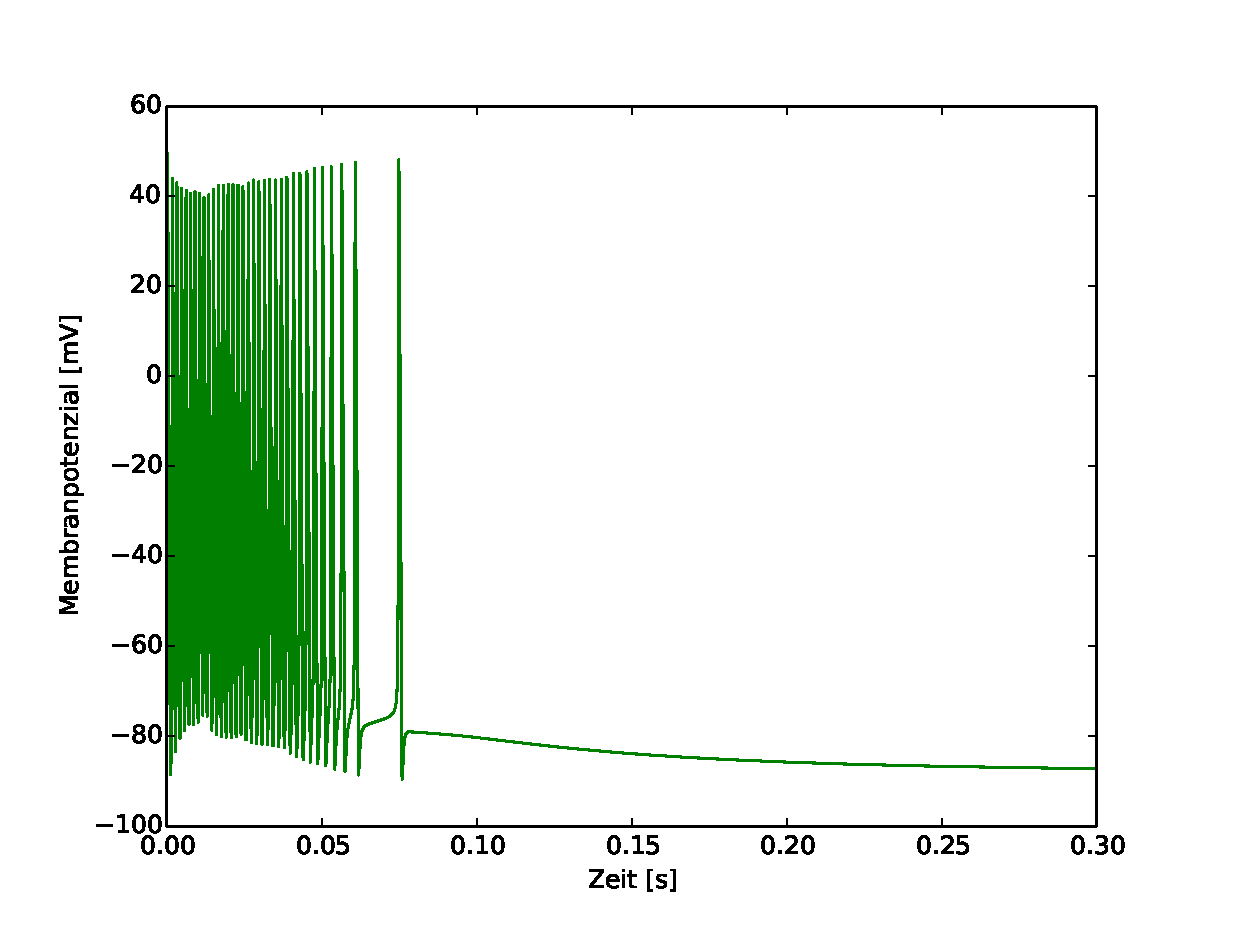
\includegraphics[viewport=19 10 532 394,width=0.35\linewidth]{genetic/rs-base.eps}
    \caption*{Mutationsstärke 15 \%}
    \begin{subfigure}{.5\textwidth}
      \centering
      \includegraphics*[viewport=19 10 532 394,width=0.7\linewidth]{genetic/rs-mut008333.eps}
      \caption*{Mutationsstärke 8.333 \%}
    \end{subfigure}%
    \begin{subfigure}{.5\textwidth}
      \centering
      \includegraphics*[viewport=19 10 532 394,width=0.7\linewidth]{genetic/rs-mut025.eps}
      \caption*{Mutationsstärke 25 \%}
    \end{subfigure}
  \end{figure}
\end{frame}

\begin{frame}
  \frametitle{Intrinsic Bursting}
  \begin{figure}
    \centering
    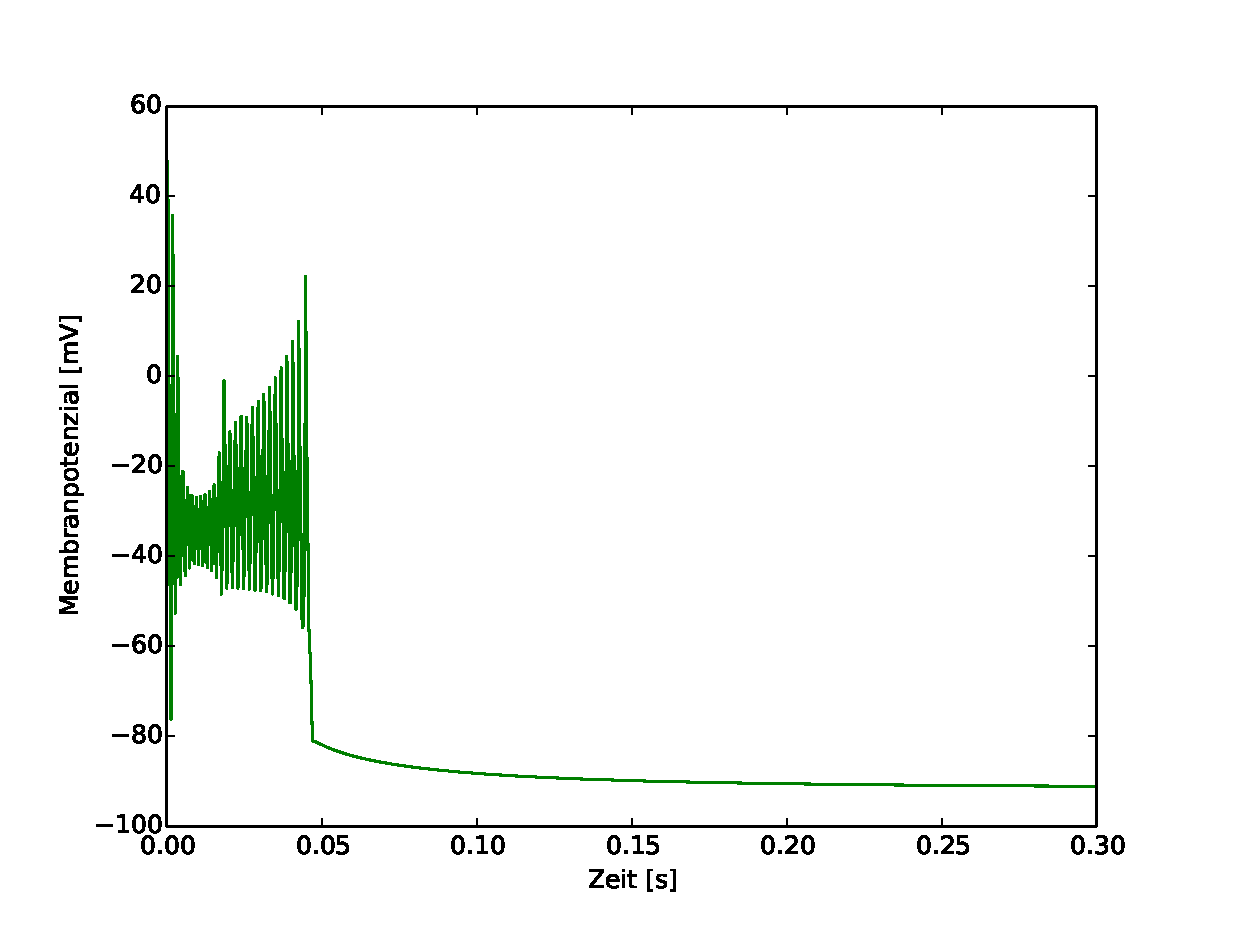
\includegraphics[viewport=19 10 532 394,width=0.35\linewidth]{genetic/ib-pop200.eps}
    \caption*{Populationsgröße 200}
    \begin{subfigure}{.5\textwidth}
      \centering
      \includegraphics*[viewport=19 10 532 394,width=0.7\linewidth]{genetic/ib-pop50.eps}
      \caption*{Populationsgröße 50}
    \end{subfigure}%
    \begin{subfigure}{.5\textwidth}
      \centering
      \includegraphics*[viewport=19 10 532 394,width=0.7\linewidth]{genetic/ib-base.eps}
      \caption*{Populationsgröße 125}
    \end{subfigure}
  \end{figure}
\end{frame}

\begin{frame}
  \frametitle{Fast Spiking}
  \begin{figure}
    \centering
    \begin{subfigure}{.5\textwidth}
      \centering
      \includegraphics*[viewport=19 10 532 394,width=0.7\linewidth]{genetic/fs-base.eps}
      \caption*{Tournament Selection (TS 5)}
    \end{subfigure}%
    \begin{subfigure}{.5\textwidth}
      \centering
      \includegraphics*[viewport=19 10 532 394,width=0.7\linewidth]{genetic/fs-tsize15.eps}
      \caption*{Tournament Selection (TS 15)}
    \end{subfigure}
  \end{figure}
  \begin{figure}
    \centering
    \begin{subfigure}{.5\textwidth}
      \centering
      \includegraphics*[viewport=19 10 532 394,width=0.7\linewidth]{genetic/fs-trunc-sel.eps}
      \caption*{Truncation Selection}
    \end{subfigure}%
    \begin{subfigure}{.5\textwidth}
      \centering
      \includegraphics*[viewport=19 10 532 394,width=0.7\linewidth]{genetic/fs-fitn-prop.eps}
      \caption*{Fitness-Proportionate Selection}
    \end{subfigure}
  \end{figure}
\end{frame}

\subsection{Aussicht}

\begin{frame}
  \begin{itemize}
  \item Kombination von zielführenden Parametern
  \item Anpassung der Fitnessfunktion
  \item mehrfache Ausführung der Läufe
  \end{itemize}
\end{frame}
\begin{frame}
\frametitle{Simulated Annealing}
    \begin{itemize}
        \item Startposition: Zufällige Werte
        \item Bestimmung der Nachbarn:
        \item Metropolis-Funktion:
    \end{itemize}
\end{frame}

\begin{frame}
\frametitle{Einstellbare Parameter}
    \begin{itemize}
        \item maxsteps
        \item start\_temperature
        \item cooling\_schedule
        \item cooling\_schdule\_alpha
        \item neighbour\_count
    \end{itemize}
\end{frame}

\begin{frame}
\frametitle{Ergebnisse}

  test frame simulated annealing and grid search
\end{frame}

\begin{frame}
\frametitle{Mögliche Verbesserungen}
    \begin{itemize}
        \item Übergeben eines Startchromosoms
        \item Erweiterung der Nachbarschaftssuche
            \begin{itemize}
                \item Mehrere Kanäle gleichzeitig verändern
                \item Konstante Schrittweite der Kanalwerte
            \end{itemize}
    \end{itemize}
\end{frame}


\end{document}
